%FILL IN THE RIGHT INFO.
%\lecture{**LECTURE-NUMBER**}{**DATE**}
\unchapter{Lecture 10}
\lecture{10}{October 6}
\setcounter{section}{0}
\setcounter{theorem}{0}

% **** YOUR NOTES GO HERE:

We go into more depth on isolated singularities of functions.


Let $\oic$ open, $z_0 \in \om$, $f: \omP \to \C$ holomorphic. Then $z_0$ is a possible isolated singularity of $f$.


\begin{definition}[Singularity]

Let $\oic$ open, $z_0 \in \om$, $f: \omP \to \C$ holomorphic. $z_0$ is said to be a \textbf{singularity }of $f$ if $f$ cannot be extended to a holomorphic function over all of $\om$ (especially at $z_0$).

\end{definition}


\begin{theorem}
Let $0 \leq r < R $. Consider $A = \set{ z\in \C \, \mid \, r< \abs{z-z_0} <R }$ (when $r=0$ this gives you a punctured disk). Let $f: A \to \C$ holomorphic. Then for every $r<r'<R'<R$, we can write $f$ as a Laurent series:

\begin{align*}
    f(z) = \sum_{-\infty}^\infty a_n (z-z_0)^n
\end{align*}
for $r' \leq \abs{z-z_0} \leq R'$, and this series is absolutely convergent on this smaller annulus $\set{ z\in \C \, \mid \, r'< \abs{z-z_0} <R' }$ and $\forall u \in (r,R)$:

\begin{align*}
    a_n = \frac{1}{2 \pi i} \int_{\abs{z-z_0}=u} \frac{f(w)}{(w-z_0)^{n+1}} \dif w
\end{align*}
\end{theorem}


\begin{center}
\begin{tikzpicture}[scale = 1.5]
    \draw[shift={(-2.5,-2)},rotate=0][dotted][scale =2.5] plot [smooth cycle] coordinates {(0,0) (1,0.1) (2,0.3) (2,0.7) (1.5,1.5) (0.8,1.5) (0.3,1.2) (-0.2,0.6) };
    
    
    \draw [pattern=north west lines][dotted][thick]  (0,0) circle (1.4);
    \draw [fill=white][dotted][thick]  (0,0) circle (0.6);
    
    \draw (0,0) -- (-40:1.4);
    \draw (0,0) -- (40:0.6);
    
    \draw[above left] (40:0.3) node {$r$};
    \draw[->] (0: 1.8) to [out=190,in=40] (-40:1);
    \draw[above] (0: 1.8) node {$R$};
    
    \draw[fill] (0,0) circle (0.02);
    \draw[left] (0,0) node {$z_0$};
    
\end{tikzpicture}    
\end{center}


\begin{note}
When we say that $\sum_{-\infty}^\infty a_n (z-z_0)^n$ is absolutely convergent we mean that both $\sum_{0}^\infty a_n (z-z_0)^n$ and $\sum_{-\infty}^0 a_n (z-z_0)^n$ are absolutely convergent.
\end{note}

\begin{example}
Consider $f(z) = e^{\frac{1}{z}}$ on $\C^* = \C \setminus \{ 0 \}$. The Laurent series on any annulus $\set{r < \abs{z} < R}$ is given by:

\begin{align*}
    f(z) = \sum_{n=0}^\infty \frac{z^{-n}}{n!}
\end{align*}

\end{example}

\begin{proof}
On smaller annulus, $f$ is holomorphic by assumption, so we apply Cauchy's integral formula. Noting that $r' \leq \abs{z-z_0} \leq R'$:








\begin{center}
\begin{tikzpicture}[decoration={
    markings,
    mark=at position 0.5 with {\arrow{>}}}
    ]
    
    \draw [dotted] (0,0) circle [radius=2.8];
    \draw[postaction={decorate}][pattern=north west lines][rotate = -120] (0,0) circle [radius=2.4];
    
    \draw[postaction={decorate}][fill = white][xscale=-1][rotate = -60] (0,0) circle [radius=1.2];
    \draw [dotted] (0,0) circle [radius=1];
    
    
    \draw[above left] (40:0.6) node {$r'$};
    
    \draw[above] (0: 3.6) node {$R'$};
    
    \draw[fill] (0,0) circle (0.02);
    \draw[left] (0,0) node {$z_0$};
    \draw[->] (0: 3.6) to [out=190,in=40] (-40:2);
    \draw (0,0) -- (-40:2.4);
    \draw (0,0) -- (40:1.2);
    
\end{tikzpicture}
\end{center}















\begin{align*}
    f(z) &= \frac{1}{2 \pi i} \int_{\abs{w- z_0} = R} \frac{f(w)}{w-z} \dif w - \frac{1}{2 \pi i} \int_{\abs{w- z_0} = r} \frac{f(w)}{w-z} \dif w
\end{align*}
using the fact that $w-z = w-z_0 -(z-z_0) = (z-z_0) \left( \frac{w-z_0}{z-z_0} -1 \right)$:

\begin{align*}
    f(z) &= \sum_{n=0}^\infty a_n (z-z_0)^n - \frac{1}{2 \pi i} \int_{\abs{w- z_0} = r} \frac{f(w)}{w-z} \dif w\\
    \text{with } a_n &= \frac{1}{2 \pi i} \int_{\abs{w- z_0} = R} \frac{f(w)}{(w-z_0)^{n+1}} \dif w
\end{align*}
Note that we cannot use the same trick for the second term since $f$ is not holomorphic inside the disk (so the power series does not converge in it). We can still do something similar. Noting that:


\begin{center}
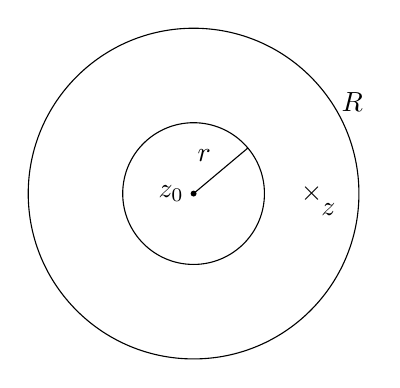
\begin{tikzpicture}[scale = 1.5]

    
    
    \draw  (0,0) circle (1.4);
    \draw [fill=white]  (0,0) circle (0.6);
    
    \draw (0,0) -- (40:0.6);
    
    \draw[above left] (40:0.3) node {$r$};
    \draw (30: 1.55) node {$R$};
    
    \draw[fill] (0,0) circle (0.02);
    \draw[left] (0,0) node {$z_0$};
    
    \draw[below right] (0: 1) node {$z$};
    \draw (0: 1) node {$\times$};
    
\end{tikzpicture}    
\end{center}




\begin{align*}
    w-z &= - (z-z_0) \left(   1-  \frac{w-z_0}{z-z_0} \right)\\
\text{and that } \abs{\frac{w-z_0}{z-z_0}} &\leq \frac{r}{r'} < 1
\end{align*}

We get that:

\begin{align*}
    -\frac{1}{w-z} &= \frac{1}{z-z_0} \cdot \frac{1}{1-\frac{w-z_0}{z-z_0}}\\ &= \frac{1}{z-z_0} \cdot \sum_{n=0}^\infty \left( \frac{w-z_0}{z-z_0} \right)^n\\
    &= \sum_{n=0}^\infty \frac{(w-z_0)^n}{(z-z_0)^{n+1}}\\
    \text{(relabel) } &= \sum_{n=0}^{-\infty} \frac{(z-z_0)^{n-1}}{(w-z_0)^n}\\
    \text{(relabel) } &= \sum_{n=-1}^{-\infty} \frac{(z-z_0)^{n}}{(w-z_0)^{n+1}}
\end{align*}

This new representation of $\frac{-1}{w-z}$ has strictly negative powers of $(z-z_0)$, exactly what we want:

\begin{align*}
    f(z) &= \sum_{n=0}^\infty a_n (z-z_0)^n - \frac{1}{2 \pi i} \int_{\abs{w- z_0} = r} \frac{f(w)}{w-z} \dif w\\
    &= \sum_{n=0}^\infty a_n (z-z_0)^n + \sum_{n=-1}^{-\infty} a_n (z-z_0)^n\\
\end{align*}
Where the $a_n$ in the second part of the sum comes from the same formula that gave us $a_n$ in the first part of the sum: $a_n = \frac{1}{2 \pi i} \int_{\abs{w- z_0} = r} \frac{f(w)}{(w-z_0)^{n+1}} \dif w$. Note that you can use any radius you want that is in the annulus, especially $r$ and $R$. The integral evaluates to the same thing by Cauchy's Theorem.
\end{proof}


\begin{remark}
In the case of poles we get the same Laurent series that we had before (ie $\sum_{-N}^\infty a_n (z-z_0)^n$). This theorem says that for a general holomorphic function the index of the sum can extend backwards to $-\infty$.
\end{remark}


Laurent series allow us to study isolated singularities. 

\section{Classification of Singularities}
\isubsection{THM: Riemann Extension Theorem}
\begin{theorem}[Riemann Extension Theorem]
Let $\oic$ open , $z_0\in \om$, $f: \omP \to \C$ holomorphic. Suppose that $\sup_{\omP}\abs{f} < \infty$. Then $\exists ! \Tilde{f}: \om \to \C$ holomorphic s.t. $\Tilde{f}\mid_{\omP} = f$.
\end{theorem}
\begin{definition}[Removable Singularities and Holomorphic Extensions]


We call this $\Tilde{f}$ a \textbf{holomorphic extension} of $f$ across $z_0$, and we will say that $z_0$ is a \textbf{removable singularity} of $f$.

\end{definition}



\begin{remark}
If $\Tilde{f}: \om \to \C$ holomorphic and we call $f=\Tilde{f}\mid_{\omP}$ then obviously $\sup_{D_r(z_0)\setminus \{z_0\} } \abs{f} < \infty$ for $r$ small.

Thus boundedness of $\, \abs{f}$ is necessary and sufficient for $z_0$ being a removable singularity.
\end{remark}

\begin{proof}
Let $R>0$ small enough that $D_R(z_0) \ssubset \om$, and so $\abs{f(z) } \leq C$ for some $C>0$, $\forall z$ such that $0 < \abs{z-z_0} < R$. Expand $f$ in Laurent series on this annulus:

\begin{align*}
    f(z) &= \sum_{-\infty}^\infty a_n (z-z_0)n\\
    \text{with } a_n &= \int_{\abs{w-z_0} = R} \frac{f(w)}{(w-z_0)^{n+1}} \dif w
\end{align*}

So for $n = -m$, $m > 0$ (ie $n<0$):

\begin{align*}
    \abs{a_{-m}} &\leq \frac{1}{2 \pi } \cdot \abs{\int_{\abs{w-z_0} =R} \frac{f(w)}{(w-z_0)^{-m+1}}  \dif w}\\
    &= \frac{1}{2 \pi } \cdot \abs{\int_{\abs{w-z_0} =R} f(w)(w-z_0)^{m-1}  \dif w}\\
    \text{let ($w(t) = z_0 +Re^{it}$) } &= \abs{\int_{\abs{w-z_0} =R} f(z_0 +Re^{it})R^{m-1} +Re^{i(m-1)t} Ri e^{it}  \dif t}\\
    &\leq R^m \cdot C \xrightarrow[]{R\to 0} 0
\end{align*}

Where the final line comes from the fact that $\abs{f}$ is bounded, and the fact that $\abs{e^{ix}} = 1$. Thus letting $R \to 0$ we get that $\abs{a_{-m}} = 0 \, \forall m>0$. Thus the Laurent series has no negative powers.

Let $\Tilde{f}(z) = \sum_{n=0}^\infty a_m (z-z_0)^n$ on $D_R(z_0)$. This agrees with $f$ on $D_R(z_0) \setminus \{ z_0 \}$, so we get a holomorphic extension of $f$ across $z_0$. The uniqueness of $\Tilde{f}$ was already discussed (compare to analytic continuation).

\end{proof}

\begin{corollary}
$f: \omP \to \C$ holomorphic. $f$ has a pole at $z_0$ iff $\abs{f(z)} \xrightarrow[]{z \to z_0} \infty$.
\end{corollary}

\begin{proof}
\begin{enumerate}
    \item[$\Rightarrow$] By definition of pole, $\frac{1}{f(z)}$ (well-defined near $z_0$) has a zero at $z_0$. Thus $\abs{\frac{1}{f(z)}} \xrightarrow[]{z\to z_0}0$ which implies that $\abs{f(z)} \xrightarrow[]{z\to z_0} \infty$.
    
    \item[$\Leftarrow$] Since $f$ goes to infinity near $z_0$, $f(z) \neq 0$ $ \forall z \in D_r(z_0) \setminus \{ z_0 \}$ for some $r>0$ small. Thus $\frac{1}{f(z)}$ is holomorphic on $D_r(z_0) \setminus \{ z_0 \}$ and $\sup_{D_r(z_0) \setminus \{ z_0 \}} \frac{1}{\abs{f(z)}} \leq C$ since $\abs{f} \to \infty$.
    
    Since $\frac{1}{f(z)}$ is holomorphic and bounded, Riemann extension applies to it. Thus $z=z_0$ is a removable singularity of $\frac{1}{f(z)}$, and since $\abs{f} \to \infty$ then $\abs{\frac{1}{f}} \xrightarrow[]{z\to z_0} 0$. Thus the holomorphic extension of $\frac{1}{f(z)}$ at $z_0$ has vale 0. Thus $z_0$ is a pole of $f$.
\end{enumerate}
\end{proof}

We can now examine the 3 different kinds of poles.

\subsection{Types of Poles}

\begin{definition}
$z_0 \in \om$, $f: \omP \to \C$ holomorphic ($z_0$ is a singularity of $f$).

There are three mutually exclusive cases:

\begin{enumerate}
    \item $z_0$ is a \textbf{removable singularity} of $f$ $\iff$ $\abs{f} < C$ near $z_0$ (iff by Riemann extension)
    
    \item $z_0$ is a \textbf{pole} of $f$ $\iff$ $\abs{f} \xrightarrow[]{z\to z_0} \infty$
    
    \item $z_0$ is an \textbf{essential singularity} of $f$ $\iff$ $z_0$ is neither removable nor a pole
\end{enumerate}
\end{definition}

\begin{example}
$f(z) = e^{\frac{1}{z}}$ has an essential singularity at $z_0 = 0$.

Consider $\abs{e^{\frac{1}{z}}}$ as $z\to 0$.

\begin{enumerate}
    \item[$0<z \in \R$:] $e^{\frac{1}{z}} \xrightarrow[]{x \to 0} +\infty$\\
    \item[$0>z \in \R$:] $e^{\frac{1}{z}} \xrightarrow[]{x \to 0} 0$\\
    \item[$z = iy,\, y \in \R$:] $\abs{e^{\frac{-i}{y}}}$ = 1 (however the argument varies wildly)
\end{enumerate}

Thus this is neither a pole nor a removable singularity.
\end{example}

You can detect the type of singularity by examining the Laurent series:

\begin{note}
Let $f(z) = \sum_{n=-\infty}^\infty a_n (z-z_0)^n$. Three distinct cases:

\begin{enumerate}
    \item $f(z) = \sum_{n=0}^\infty a_n (z-z_0)^n$. This implies $z_0$ is a removable singularity.
    
    \item $f(z) = \sum_{n=-N}^\infty a_n (z-z_0)^n$. This implies $z_0$ is a pole.
    
    \item $f(z) = \sum_{n=-\infty}^\infty a_n (z-z_0)^n$. This implies $z_0$ is an essential singularity.
\end{enumerate}


\end{note}

\isubsection{THM: Casorati-Weierstra{\ss}}
\begin{theorem}[Casorati-Weierstra{\ss}]

Suppose $f: \omP \to \C$ holomorphic and $z_0$ an essential singularity. Then $\forall r> 0$ small such that $D_r(z_0) \subset \om$, we have that $f(D_r(z_0) \setminus \{ z_0 \})$ is dense in $\C$.
\end{theorem}

%ADD A DRAWING MAYBE? I CANNOT DRAW DENSE SETS


\begin{proof}
Suppose that $A = f(D_r(z_0) \setminus \{ z_0 \})$ is not dense. Then $\overline{A} \neq \C$. Thus $\exists w \in \C$, $w \notin \overline{A} $. Then  $w$ has positive distance from $\overline{A}$, ie $\exists \delta >0$ s.t. $\abs{f(z) - w} > \delta$, $\forall z \in A$. Let $g(z) = \frac{1}{f(z) - w}$, $z \in A$ (this is okay since we know that $\abs{f(z) - w} > 0$). This is holomorphic on $A$ with $g \neq 0$ on the punctured disk.

Then $\abs{g(z)} < \frac{1}{\delta} \, \forall z \in A$, so $z_0$ is a removable singularity for $g$. Two cases follow:


\begin{enumerate}
    \item[$g(z_0) \neq 0$:] $g(z) = \frac{1}{f(z) - w}$, $g(z) \neq 0$ near $z_0$, thus we take $\frac{1}{g(z)} + w = f(z)$. Since this is a sum of two holomorphic functions, $f$ is also holomorphic at $z_0$. Thus $z_0$ is a removable singularity of $f$. $\lightning$
    \item[$g(z_0) = 0$:] Then since $g\neq 0$,  $z_0$ is an isolated zero of $g$ with an order of vanishing of $N \geq 1$. So $f(z) = w + \frac{1}{g(z)}$. This is holomorphic on $A$ as the sum of two functions that are holomorphic on $A$. Since $\frac{1}{g(z)}$ has a pole at $z_0$, so does $f(z)$. $\lightning$
\end{enumerate}





\end{proof}



\begin{remark}
We have a trichotomy of singularities. Removable singularities are in a sense not real singularities. Poles are our friends; they have residues and we can use the residue formula on them. Essential singularities are wild and bad, and behave very badly.
\end{remark}

Poles are special enough that we give a name to functions that are composed of only poles for singularities.


\begin{definition}[Meromorphic Functions]
A function $f$ on $\om$ open is called \textbf{meromorphic} if there is a countable collection $\{ z_i \}_{i=0}^\infty \subset \om$ of points with no accumulation point inside $\om$ (the boundary is possible), and $f: \om \setminus \bigcup_{j=0}^\infty \{ z_j \} \to \C $ holomorphic function such that $z_j$'s are all poles of $f$.
\end{definition}



